\documentclass{report} 
\title{Signals And Systems by Alan V. Oppenheim:\\Notes}
\date{Started 17 April 2025}
\author{Malcolm}
\usepackage{amsmath} %import math
\usepackage{mathtools} %more math
\usepackage{amssymb} %for QED symbol
\usepackage{amsthm} %
\usepackage{bm}%bold math
\usepackage{graphicx} %import imaging
\graphicspath{{./images/}} %set imaging path
\begin{document}
\maketitle

\tableofcontents

\newpage
\section{Introduction}
\subsection{Signal Energy and Power}
\textbf{Motivation and definition}\\
In many but not all, applications, the signals considered directly related to physical quantities capturing
power and energy in a physical system. (for instance $v^2/R$ for the power across a resistor)\\
\vspace{1mm}\\
As such it is a common and worthwhile convention to use similar terminology for power and energy for \textit{any} 
continuous-time signal, denoted $x(t)$, or any discrete-time signal $x[n]$. 
In this case, the total energy over the time interval $t_1\leq t\leq t_2$ in a continuous signal $x(t)$ is defined
as
\begin{equation*}
\int^{t_2}_{t_1}|x(t)|^2dt
\end{equation*}
where $|x|$ denotes the magnitude of the (possibly complex) number $x$; see that the time-averaged signal 
can be obtained by dividing by $(t_2-t_1)$. Similarly for a discrete signal $x[n]$ over the interval $n_1\leq n\leq n_2$ the total energy is
\begin{equation*}
\sum^{n_2}_{n=n_1}|x[n]|^2
\end{equation*}
with the average power calculated by dividing by $(n_2-n_1+1)$.\\
\vspace{1mm}\\
It is important to remember that the terms `power' and `energy' are used here \textit{independently} of their 
relation to physical energy (they clearly don't correlate since their units or scalings would differ). Nevertheless
we will find it convenient to use these terms in a general fashion.\\
\vspace{1mm}\\
\textbf{Power and energy over infinite intervals}\\
Considering signals over an infinite time interval, meaning for $-\infty<t<+\infty$ or $-\infty<n<+\infty$. 
Here we define the total energy as the limits of the aforementioned equations increase without bound; in continuous
time,
\begin{equation*}
E_\infty\triangleq\lim_{T\to\infty}\int^T_{-T}|x(t)|^2dt
=\int^{+\infty}_{-\infty}|x(t)|^2dt
\end{equation*}
and in discrete time,
\begin{equation*}
E_\infty\triangleq\lim_{N\to\infty}\sum^{+N}_{n=-N}|x[n]|^2=\sum^{+\infty}_{n=-\infty}|x[n]|^2
\end{equation*}
Note that these expressions may not converge; for instance say $x(t)$ or $x[n]$ equal some nonzero constant for 
all time: such signals have infinite energy, while signals with $E_\infty<\infty$ have finite energy.\\
(next page)\newpage
\noindent\textbf{Cont.}\\
Analagously, we can define the time-averaged power over an infinite interval as
\begin{equation*}
P_\infty\triangleq\lim_{T\to\infty}\frac{1}{2T}\int^T_{-T}|x(t)|^2dt
\end{equation*}
and
\begin{equation*}
P_\infty\triangleq\lim_{N\to\infty}\frac{1}{2N+1}\sum^{+N}_{n=-N}|x[n]|^2
\end{equation*}
In continuous and discrete time respectively. \\
\vspace{1mm}\\
\textbf{Intuition}\\
See that with these definitions, we can identify three classes of signals: first those with finite total energy,
meaning $E_\infty<\infty$. See that such a signal would have zero average power:
\begin{equation*}
P_\infty=\lim_{T\to\infty}\frac{E_\infty}{2T}=0
\end{equation*}
Second would be signals with finite average power $P_\infty$; see from the above expression that for $P_\infty>0$,
this requires that $E_\infty=\infty$.\\
\vspace{1mm}\\
Last would be signals for which neither $P_\infty$ nor $E_\infty$ are finite. An example of this might be $x(t)=t$.\\
\vspace{1mm}\\
\textbf{Note on discrete signals}\\
It is important to note that the discrete-time signal $x[n]$ is defined \textit{only} for \textit{integer} 
values of the independent variable.
\newpage

\subsection{Even and Odd signals}
\textbf{Definition}\\
A continuous-time signal is \textit{even} if
\begin{equation*}
x(-t)=x(t)
\end{equation*}
while a discrete-time signal is \textit{even} if
\begin{equation*}
x[-n]=x[n]
\end{equation*}
These signals are referred to as \textit{odd} if
\begin{align*}
x(-t)&=-x(t)\\
x[-n]&=-x[n]
\end{align*}
Note that an odd signal must be 0 at $t=0$ or $n=0$ since the equations require that $x(0)=-x(0)$ and $x[0]=-x[0]$.
\\
\vspace{1mm}\\
\textbf{Decomposition}\\
An important fact is that any signal can be broken into a sum of two signals, where one is even and the other odd.
To see this, consider
\begin{equation*}
\text{Ev}\{x(t)\}=\frac{1}{2}[x(t)+x(-t)]
\end{equation*}
which is referred to as the \textit{even part} of $x(t)$. Similarly, the \textit{odd part} of $x(t)$ is given by
\begin{equation*}
\text{Od}\{x(t)\}=\frac{1}{2}[x(t)-x(-t)]
\end{equation*}
See that $x(t)$ is the sum of the two. Exactly analagous definitions hold in the discrete time case.
\begin{center}
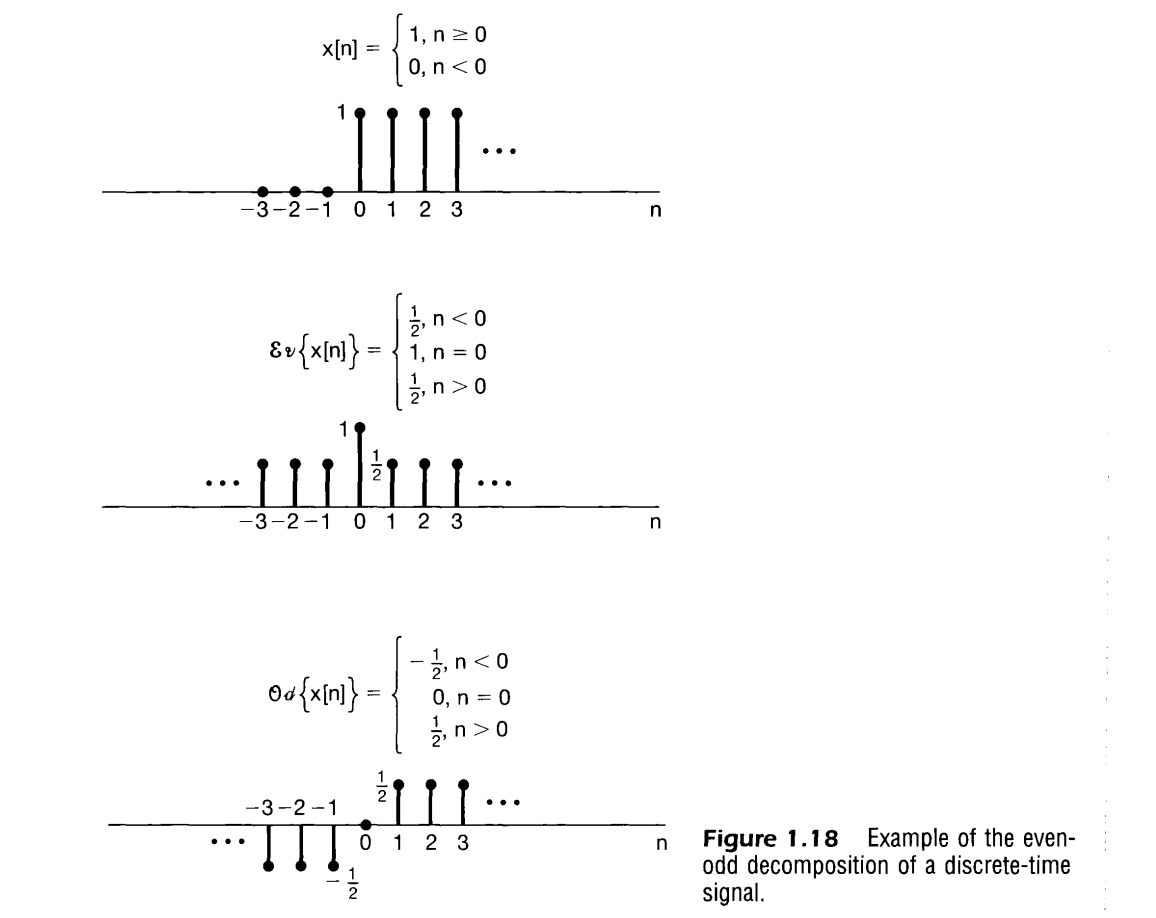
\includegraphics[width=9cm]{a1}
\end{center}
\newpage

\subsection{Differences between continuous and\\discrete periodic complex exponentials}
The continuous-time \textit{complex exponential signal} is of the form
\begin{equation*}
x(t)=Ce^{at}
\end{equation*}
where $C$ and $a$ are, in general, complex numbers. An important class of complex exponentials is obtained by constraining $a$ to be purely imaginary:
\begin{equation*}
x(t)=e^{i\omega t}
\end{equation*}
\textbf{Periodicity and harmonic relations (purely imaginary power)}\\
An important property of this signal is that it is periodic; recall that $x(t)$ will be periodic with period $T$ if
\begin{equation*}
e^{i\omega t}=e^{i\omega(t+T)}
\end{equation*}
this means
\begin{equation*}
e^{i\omega(t+T)}=e^{i\omega t}e^{i\omega T}\implies
e^{i\omega T}=1
\end{equation*}
If $\omega=0$ then this is satisfied for any $T$. If $\omega\neq0$, see that the \textit{fundamental period} 
$T_0$ of $x(t)$---that is, the smallest positive value of $T$ for which this holds---is
\begin{equation*}
T_0=\frac{2\pi}{|\omega|}
\end{equation*}
(the signals $e^{i\omega 0t}$ and $e^{-i\omega t}$ have the same fundamental period)
Naturally, there is a set of exponentials periodic to a common period $T_0$. These are said to be
\textit{harmonically related} complex exponentials; the necessary condition they satisfy is
\begin{equation*}
e^{i\omega T_0}=1
\end{equation*}
which implies that
\begin{equation*}
\omega T_0=2\pi k,\quad k=0,\pm1,\pm2,\ldots
\end{equation*}
(next page)\newpage
\noindent\textbf{Cont.}\\
We had
\begin{equation*}
\omega T_0=2\pi k,\quad k=0,\pm1,\pm2,\ldots
\end{equation*}
if we define
\begin{equation*}
\omega_0=\frac{2\pi}{T_0}
\end{equation*}
this means that the harmonic frequencies $\omega$ must be integer multiples of $\omega_0$:
\begin{equation*}
\phi_k(t)=e^{ik\omega_0t},\quad k=0,\pm1,\pm2,\ldots
\end{equation*}
For $k=0$, $\phi_k(t)$ is a constant, while for any other value of $k$, $\phi_k(t)$ is periodic with fundamental 
frequency $|k|\omega_0$ and fundamental period
\begin{equation*}
\frac{2\pi}{|k|\omega_0}=\frac{T_0}{|k|}
\end{equation*}
Each $\phi_k(t)$ itself defines a fundamental frequency and a corresponding fundamental period. 
(see that $|k|\omega_0\cdot T_0/|k|=2\pi$, so this scaled down period is the corresponding period
for this scaled up frequency. Each frequency is unique, point here is that they are also periodic with $T_0$, 
but with fundamental periods getting proportionally smaller.)\\
\vspace{1mm}\\
Note that the $k$th harmonic $\phi_k(t)$ is still periodic with $T_0$; it goes through exactly $|k|$ of its 
fundamental periods during any time interval of length $T_0$. (the term `harmonic' is consistent with its use in
music, where it refers to tones resulting from variations in acoustic pressure at frequencies that are integer
multiples of a fundamental frequency)\\
(next page)\newpage
\noindent\textbf{Discrete case}\\
As in continuous time, an important signal in discrete time is the \textit{complex exponential signal}, defined as
\begin{equation*}
x[n]=C\alpha^n
\end{equation*}
where $C$ and $\alpha$ are, in general, complex numbers. See that this could also be expressed as
\begin{equation*}
x[n]=Ce^{\beta n}
\end{equation*}
where $\alpha=e^\beta$. See that we can constrain $\beta$ to be purely imaginary:
\begin{equation*}
x[n]=e^{i\omega_0n}
\end{equation*}
\textbf{Periodicity properties of Discrete-time complex exponentials}\\
While there are many similarities between continuous and discrete-time signals, there are a number of important
differences. For the continuous time signal $e^{i\omega_0t}$, we know that
\begin{itemize}
\item The larger the magnitude of $\omega_0$, the higher the rate of oscillation of the signal
\item $e^{i\omega_0t}$ is periodic for any value of $\omega_0$
\end{itemize}
These properties are different in the discrete-time case.\\
\vspace{1mm}\\
Given the first property, consider the discrete-time complex exponential with frequency $\omega_0+2\pi$:
\begin{equation*}
e^{i(\omega_0+2\pi)n}=e^{i2\pi n}e^{i\omega_0n}=e^{i\omega_0n}
\end{equation*}
(see that this is a direct result of the fact that we iterate through discrete time as integers) 
The exponential at frequency $\omega_0+2\pi$ is the \textit{same} as that at frequency $\omega_0$. 
This is unlike the continuous-time case where each distinct $\omega_0$ represents a distinct signal.\\
\vspace{1mm}\\
In discrete time, the signal with frequency $\omega_0$ is identical to the signals with frequencies 
$\omega_0\pm2\pi,\omega_0\pm4\pi$, and so on. Therefore when considering discrete time complex exponentials, 
see that we need only consider a frequency interval of length $2\pi$ in which to choose $\omega_0$, such as 
$0\leq\omega_0<2\pi$ or $-\pi\leq\omega_0<\pi$.\\
\vspace{1mm}\\
Also see that because of this the discrete exponential 
$e^{i\omega_0n}$ does \textit{not} have a continually 
increasing rate of oscillation as $\omega_0$ increases in magnitude; the signals will oscillate faster until we 
reach $\omega_0=\pi$, after which the rate of oscillation decreases until we reach $\omega_0=2\pi$, at which 
the same constant sequence as $\omega_0=0$ is produced.\\
(next page)\newpage
\noindent\textbf{Cont.}\\
The second property we wish to consider concerns the periodicity of the discrete time complex exponential. In
order for the signal $e^{i\omega_0n}$ to be periodic with
period $N>0$ we must have
\begin{equation*}
e^{i\omega_0(n+N)}=e^{i\omega_0n}
\end{equation*}
or equivalently 
\begin{equation*}
e^{i\omega_0N}=1
\end{equation*}
For this to hold, $\omega_0N$ must be a multiple of $2\pi$. That is, there must be an integer $m$ such that
\begin{equation*}
\omega_0N=2\pi m
\end{equation*}
or equivalently
\begin{equation*}
\frac{\omega_0}{2\pi}=\frac{m}{N}
\end{equation*}
The signal $e^{i\omega_0n}$ is periodic if $\omega_0/2\pi$ is a rational number and is not periodic otherwise.\\
\vspace{1mm}\\
\textbf{Fundamental period}\\
Recall the idea of a \textit{fundamental period}; in this case it would mean the smallest $N$ such that 
$\omega_0N=2\pi m$ holds (this is unlike the continuous case where there is always some $T$ where $\omega_0T=2\pi$); see that this occurs when $m$ and $N$ do not have any factors in common.\\
\vspace{1mm}\\
See that from this we can derive a \textit{fundamental frequency} as
\begin{equation*}
\frac{2\pi}{N}=\frac{\omega_0}{m}
\end{equation*}
(see that this frequency is always equal or lower---intuitively, to have a different wave that completes one
oscillation in $N$ time, its frequency will either be equal or lower)\\
\vspace{1mm}\\
To summarize
\begin{center}
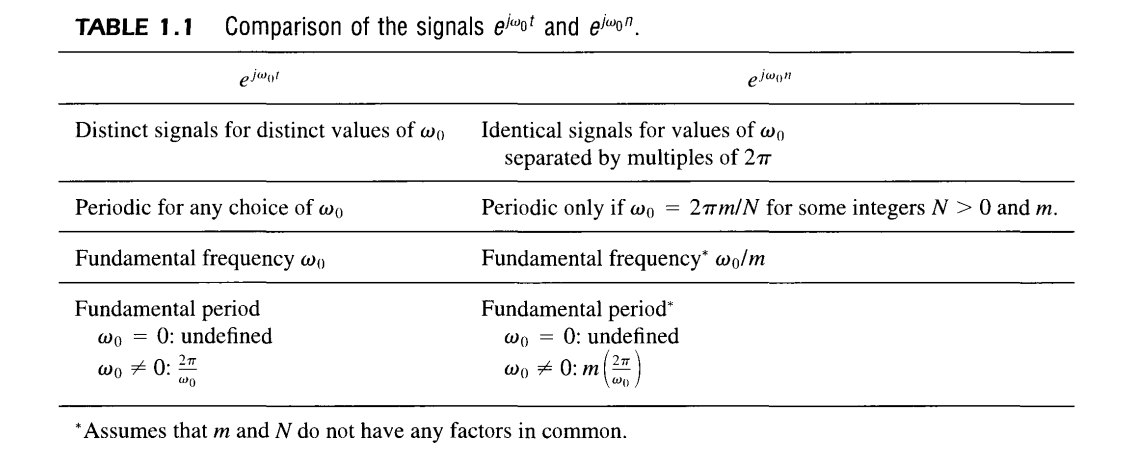
\includegraphics[width=10cm]{a2}
\end{center}
\newpage

\subsection{Intuition for discrete-time periodicity}
Consider the sequence $x[n]=\cos(2\pi n/12)$:
\begin{center}
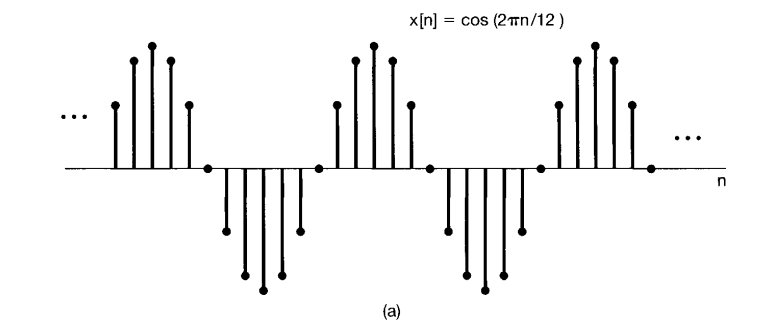
\includegraphics[width=10cm]{a3}
\end{center}
we can think of this as a set of samples of the continuous-time sinusoid $x(t)=\cos(2\pi t/12)$ at integer time
points. In this case, see that both $x(t)$ and $x[n]$ are periodic with fundamental period 12.
That is, the values of $x[n]$ repeat every 12 points, exactly in step with the fundamental period of $x(t)$.\\
\vspace{1mm}\\
Now consider the signal $x[n]=\cos(8\pi n/31)$:
\begin{center}
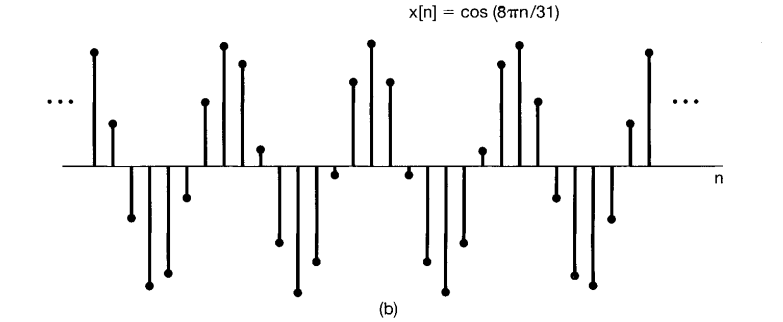
\includegraphics[width=10cm]{a4}
\end{center}
This can also be viewed as a set of samples of $x(t)=\cos(8\pi t/31)$ at integer points in time. 
But now see that in this case $x(t)$ is periodic with fundamental period $31/4$, while $x[n]$ is periodic with 
fundamental period 31.\\
\vspace{1mm}\\
This difference stems from the fact that the discrete-time signal is defined only for integer values of the 
independent variable---there is no sample at time
$t=31/4$, when $x(t)$ completes one period, or at $t=2\cdot31/4$ or $t=3\cdot31/4$, when $x(t)$ has completed two
or three periods. Only at sample $t=4\cdot31/4=31$, when
$x(t)$ has completed \textit{four} periods is the discrete sequence defined.\\
\vspace{1mm}\\
This manifests as the pattern of $x[n]$ not repeating with each cycle of positive and negative values, but rather
only after four of such cycles, specifically 31 points.\\
(next page)\newpage
\noindent\textbf{Cont.}\\
Finally consider the signal $x[n]=\cos(n/6)$:
\begin{center}
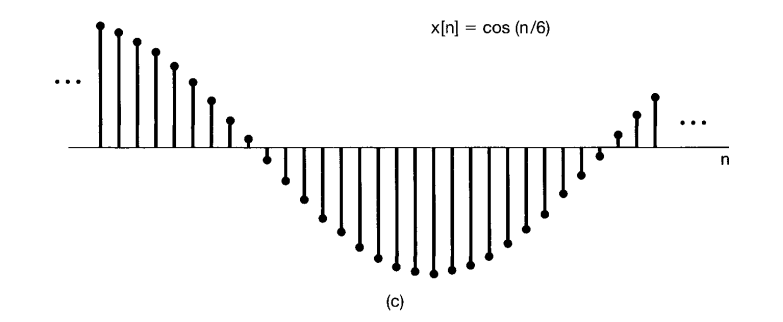
\includegraphics[width=10cm]{a5}
\end{center}
In this case, the values of $x(t)$ at integer sample points \textit{never repeat}, as these sample points never
span an interval that is an exact multiple of the period,
$12\pi$, of $x(t)$.\\
\vspace{1mm}\\
Thus, $x[n]$ \textit{is not periodic}, although the eye visually interpolates between the sample points,
suggesting \textit{the envelope} $x(t)$ which is periodic.
\newpage

\subsection{Difference in harmonic relations in discrete and\\continuous periodic exponentials}
As in continuous time, it is also of considerable value in discrete-time to consider sets of harmonically related
periodic exponentials---that is, \textit{periodic exponentials with a common period $N$}.\\
\vspace{1mm}\\
We know that these are precisely the signals which are at frequencies which are multiples of $2\pi/N$; that is
\begin{equation*}
\phi_k[n]=e^{ik(2\pi/N)n},\quad k=0,\pm1,\ldots
\end{equation*}
In the continuous-time case, all the harmonically related complex exponentials 
$e^{ik(2\pi/T_0)t},\,k=0,\pm1,\pm2,\ldots$ are distinct.
However, recall that for discrete signals we have
\begin{equation*}
e^{i(\omega_0+2\pi)n}=e^{i2\pi n}e^{i\omega_0n}=e^{i\omega_0n}
\end{equation*}
(this is a direct result of the fact that we iterate through discrete time as integers) As such the harmonically
related complex exponentials \textit{are not all unique in discrete time}; specifically,
\begin{align*}
\phi_{k+N}[n]&=e^{i(k+N)(2\pi/N)n}\\
&=e^{ik(2\pi/N)n}e^{i2\pi n}=\phi_k[n]
\end{align*}
See that this implies that there are only $N$ distinct 
periodic exponentials in the set of $\phi_k[n]$; meaning
\begin{equation*}
\phi_0[n]=1,\,\phi_1[n]=e^{i(2\pi/N)n},\,
\phi_2[n]=e^{i2(2\pi/N)n},\ldots,\,
\phi_{N-1}[n]=e^{i(N-1)(2\pi/N)n}
\end{equation*}
are all distinct, but any other $\phi_k[n]$ would just be identical to one of them. (for instance $\phi_N[n]=\phi_0[n]$ or $\phi_{-1}[n]=\phi_{N-1}[n]$.)
\newpage

\subsection{More on complex exponential and sinusoidal signals}
\textbf{Continuous case}\\
A continuous-time \textit{complex exponential signal} is of the form 
\begin{equation*}
x(t)=Ce^{at}
\end{equation*}
where $C$ and $a$ are, in general, complex numbers.\\
\vspace{1mm}\\
\textbf{Euler identity and `combined' sinusoidal form}\\
Recall euler's identity:
\begin{equation*}
e^{i\omega_0t}=\cos(\omega_0t)+i\sin(\omega_0t)
\end{equation*}
See that the scaled and phase-delayed sinusoid can be written in terms of these periodic complex exponentials
with the same fundamental period:
\begin{equation*}
A\cos(\omega_0t+\phi)=\frac{A}{2}e^{i\phi}e^{i\omega_0t}
+\frac{A}{2}e^{-i\phi}e^{-i\omega_0t}
\end{equation*}
We can also express
\begin{equation*}
A\cos(\omega_0t+\phi)=A\text{Re}\{e^{i(\omega_0t+\phi)}\}
\end{equation*}
and
\begin{equation*}
A\sin(\omega_0t+\phi)=A\text{Im}\{e^{i(\omega_0t+\phi)}\}
\end{equation*}
\textbf{Energy and power}\\
Periodic signals---and in particular, the complex periodic exponential signal---are examples of signals
with infinite total energy but finite average power. 
Calculating the total energy and of the periodic exponential signal over one period:
\begin{align*}
E_{\text{period}}&=\int^{T_0}_0|e^{i\omega_0t}|^2dt\\
&=\int^{T_0}_01\,dt=T_0
\end{align*}
(The absolute value of a complex number is its magnitude. Think of the absolute value as the 
(possibly multidimensional) distance from zero.) Calculating the average power:
\begin{equation*}
P_{\text{period}}=\frac{1}{T_0}E_{\text{period}}=1
\end{equation*}
Since there are an infinite number of periods as $t$ ranges from $-\infty$ to $+\infty$, the total energy 
integrated over all time is infinite.
However, since the average power over each period is 1, averaging over multiple periods always yields an average
power of 1. That is, the complex periodic exponential
signal has finite average power equal to
\begin{equation*}
P_\infty=\lim_{T\to\infty}\frac{1}{2T}\int^T_{-T}|e^{i\omega_0t}|^2dt=1
\end{equation*}
(next page)\newpage
\noindent\textbf{General continuous complex exponential signals}\\
In the most general case $Ce^{at}$ where both $C$ and $a$ are complex, see that since $C$ and $a$ can are just
\begin{equation*}
C=|C|e^{i\theta},\quad a=r+i\omega_0
\end{equation*}
we can express the general complex signal as
\begin{equation*}
Ce^{at}=|C|e^{i\theta}e^{(r+i\omega_0)t}=|C|e^{rt}e^{i(\omega_0t+\theta)}
\end{equation*}
we can expand this further as
\begin{equation*}
Ce^{at}=|C|e^{rt}\cos(\omega_0t+\theta)+i|C|e^{rt}\sin(\omega_0t+\theta)
\end{equation*}
\textbf{Discrete case}\\
As in continuous time, the discrete time \textit{complex exponential signal} is defined by
\begin{equation*}
x[n]=C\alpha^n
\end{equation*}
where $C$ and $\alpha$ are, in general, complex numbers. This could alternatively be expressed in the form
\begin{equation*}
x[n]=Ce^{\beta n}
\end{equation*}
where $\alpha=e^{\beta}$.\\
\vspace{1mm}\\
\textbf{Euler identity and `combined' sinusoidal form}\\
As with the continuous case, constraining $\beta$ to be
purely imaginary, we have euler's identity
\begin{equation*}
e^{i\omega_0n}=\cos\omega_0n+i\sin\omega_0n
\end{equation*}
and 
\begin{equation*}
A\cos(\omega_0n+\phi)=\frac{A}{2}e^{i\phi}e^{i\omega_0n}+
\frac{A}{2}e^{-i\phi}e^{-i\omega_0n}
\end{equation*}
\textbf{General discrete complex exponential signals}\\
As with the continuous case, for complex $C$ and $\alpha$, we have
\begin{equation*}
C=|C|e^{i\theta},\quad\alpha=|\alpha|e^{i\omega_0}
\end{equation*}
so the general complex exponential signal can be expressed as
\begin{equation*}
C\alpha^n=|C||\alpha|^n\cos(\omega_0n+\theta)
+i|C||\alpha|^n\sin(\omega_0n+\theta)
\end{equation*}
\newpage

\subsection{Unit impulse and Unit step functions}
\textbf{Discrete-Time}\\
One of the simplest discrete-time signals is the \textit{unit impulse}/\textit{unit sample}, defined as
\begin{equation*}
\delta[n]=\begin{cases}0,&n\neq0\\
1,&n=0\end{cases}
\end{equation*}
\begin{center}
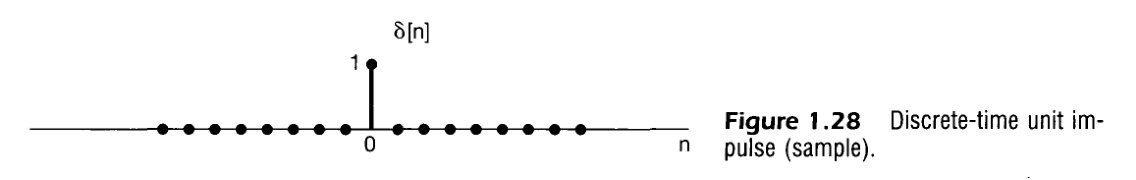
\includegraphics[width=10cm]{a6}
\end{center}
Another basic discrete-time signal is the discrete-time \textit{unit step}, denoted by $u[n]$ and defined by
\begin{equation*}
u[n]=\begin{cases}
0,&n<0\\
1,&n\geq0\end{cases}
\end{equation*}
\begin{center}
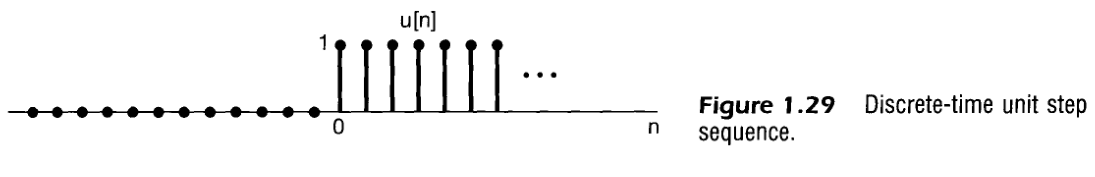
\includegraphics[width=10cm]{a7}
\end{center}
See that the discrete-time unit impulse is the \textit{first difference} of the discrete-time step:
\begin{equation*}
\delta[n]=u[n]-u[n-1]
\end{equation*}
Conversely, the discrete-time unit step is the \textit{running sum} of the unit sample:
\begin{equation*}
u[n]=\sum^n_{m=-\infty}\delta[m]
\end{equation*}
\begin{center}
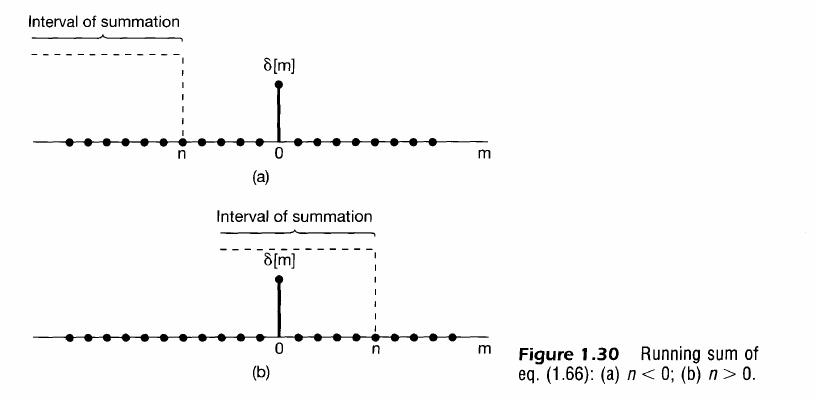
\includegraphics[width=10cm]{a8}
\end{center}
Since the only nonzero value of the unit sample is at 0, the running sum is 0 for $n<0$ and 1 for $n\geq0$.\\
(next page)\newpage
\noindent\textbf{Alternative form}\\
we had the discrete-time unit step as the running sum of the unit sample:
\begin{equation*}
u[n]=\sum^n_{m=-\infty}\delta[m]
\end{equation*}
See that by changing the variable of summation from $m$ to $k=n-m$, we can rewrite this as
\begin{equation*}
u[n]=\sum^0_{k=\infty}\delta[n-k]
\end{equation*}
and equivalently
\begin{equation*}
u[n]=\sum^\infty_{k=0}\delta[n-k]
\end{equation*}
An interpretation of this is a superposition of delayed impulses; we can view the unit step as the sum of unit impulses $\delta[n]$
(nonzero at $n=0$), $\delta[n-1]$ (nonzero at $n=1$), and all other $\delta[n-k]$ for integer $k$ extending to infinity.\\
\vspace{1mm}\\
\textbf{Sampling property}\\
See that the unit impulse can also be used to sample the value of a signal at $n=0$; since $\delta[n]$ is nonzero (and equal to 1)
only for $n=0$, it follows that
\begin{equation*}
x[n]\delta[n]=x[0]\delta[n]
\end{equation*}
More generally, if we consider a unit impulse $\delta[n-n_0]$ at $n=n_0$, then
\begin{equation*}
x[n]\delta[n-n_0]=x[n_0]\delta[n-n_0]
\end{equation*}
(next page)\newpage
\noindent\textbf{Continuous-Time}\\
The continuous-time \textit{unit step function} $u(t)$ is defined in a similar manner to its discrete-time counterpart:
\begin{equation*}
u(t)=\begin{cases}0,&t<0\\
1,&t>0\end{cases}
\end{equation*}
\begin{center}
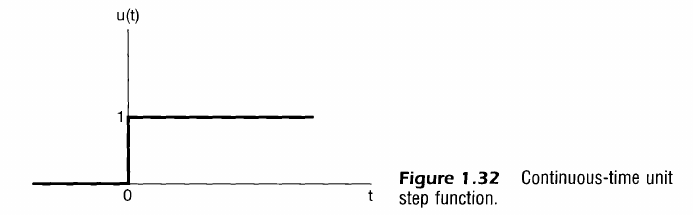
\includegraphics[width=10cm]{a9}
\end{center}
Note that the unit step is \textit{discontinuous} at $t=0$. The continuous-time \textit{unit inpulse} $\delta(t)$ is related to the
unit step in a manner analagous to that of their discrete counterparts; in particular, the continuous-time unit step is the
\textit{running integral} of the unit impulse:
\begin{equation*}
u(t)=\int^t_{-\infty}\delta(\tau)d\tau
\end{equation*}
It also follows that the continuous-time unit impulse can be thought of as the \textit{first derivative} of the continuous-time unit step:
\begin{equation*}
\delta(t)=\frac{du(t)}{dt}
\end{equation*}
In contrast to discrete-time, there is some formal difficulty with this equation as a representation of the unit impulse---since $u(t)$ is 
discontinuous at $t=0$ and consequently is not formally differentiable.\\
(next page)\newpage 
\noindent\textbf{Cont.}\\
We get around this by considering an approximation to the unit step
$u_\Delta(t)$, rising from the value 0 to 1 in a short time interval of
length $\Delta$:
\begin{center}
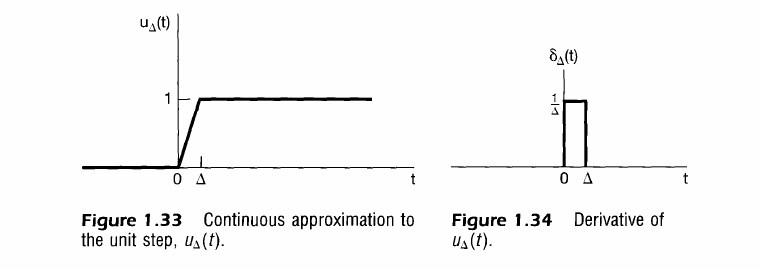
\includegraphics[width=10cm]{a10}
\end{center}
Also considering the derivative:
\begin{equation*}
\delta_\Delta(t)=\frac{du_\Delta(t)}{dt}
\end{equation*}
The unit step changes from value 0 to 1 instantaneously and can be thought of an idealisation of $u_\Delta(t)$ for $\Delta$ so short
that its duration doesn't matter for any practical purpose.
Formally, $u(t)$ is the limit of $u_\Delta(t)$ as $\Delta\to0$.\\
\vspace{1mm}\\
Consider the derivative again; $\delta_\Delta(t)$ is a short pulse, of duration $\Delta$ and unit area for any value of $\Delta$.
As $\Delta\to0$, $\delta_\Delta(t)$ becomes narrower and higher while mantaining its unit area. Its limiting form
\begin{equation*}
\delta(t)=\lim_{\Delta\to0}\delta_\Delta(t)
\end{equation*}
can then be thought of as an idealisation of the short pulse $\delta_\Delta(t)$ as the duration $\Delta$ becomes insignificant:
\begin{center}
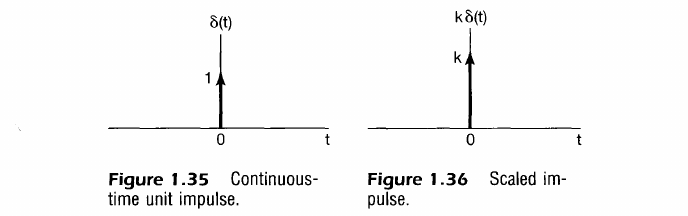
\includegraphics[width=10cm]{a11}
\end{center}
$\delta(t)$ has, in effect, no duration but unit area. The arrow at $t=0$ indicates the area of the pulse is concentrated
at $t=0$ and the height of the arrow and the `1' next to the arrow is used to represent the \textit{area} of the impulse. More generally, 
a scaled impulse $k\delta(t)$ will have an area $k$, and thus
\begin{equation*}
ku(t)=\int^t_{-\infty}k\delta(\tau)d\tau
\end{equation*}
A scaled impulse, where the height of the arrow is chosen to be proportional to the area of the impulse.\\
(next page)\newpage
\noindent\textbf{Alternative form}\\
As with discrete time, the relationship between the continuous time unit step and impulse can be rewritten in a different form, 
by changing the variable of integration from $\tau$ to $\sigma=t-\tau$:
\begin{equation*}
u(t)=\int_{-\infty}^t\delta(\tau)d\tau=\int^0_\infty\delta(t-\sigma)(-d\sigma)
\end{equation*}
or equivalently
\begin{equation*}
u(t)=\int_0^\infty\delta(t-\sigma)\,d\sigma
\end{equation*}
(This negation after inverstion of the limits of the integral can be derived from the first fundamental theorem. For a 
more intuitive understanding, consult the definition of the Riemann sum:
\begin{equation*}
\sum^{n-1}_{i=0}f(t_i)(x_{i+1}-x_{i})
\end{equation*}
Considering the $d\tau$, or respectively $d\sigma$, as the width of the step between two argumentsof the sum, if we change the
direction in which we integrate, the step also changes its sign.
In the discrete sum, the summands are not multiplied by this step.)\\
\vspace{1mm}\\
\textbf{Sampling property}\\
As with discrete-time, the continuous-time impulse has a very important sampling property; consider 
\begin{equation*}
x_1(t)=x(t)\delta_\Delta(t)
\end{equation*}
By construction, $x_1(t)$ is zero outside the interval $0\leq t\leq\Delta$. See that for $\Delta$ sufficiently small so that
$x(t)$ is approximately constant over this integral:
\begin{center}
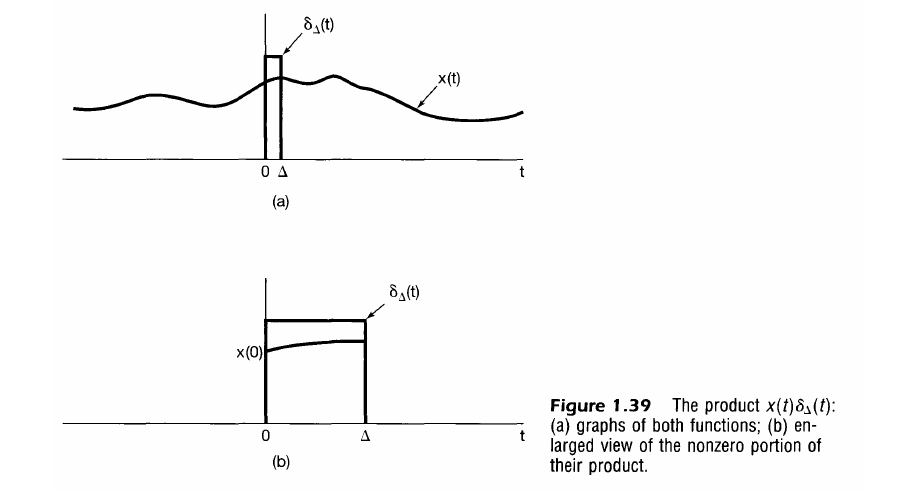
\includegraphics[width=10cm]{a12}
\end{center}
so we have
\begin{equation*}
x(t)\delta_\Delta(t)\approx x(0)\delta_\Delta(t)
\end{equation*}
(next page)\newpage
\noindent\textbf{Cont.}\\
We had, for small $\Delta$,
\begin{equation*}
x(t)\delta_\Delta(t)\approx x(0)\delta_\Delta(t)
\end{equation*}
since $\delta(t)$ is the limit as $\Delta\to0$ of $\delta_\Delta(t)$, it follows that
\begin{equation*}
x(t)\delta(t)=x(0)\delta(t)
\end{equation*}
By the same argument, we have an analagous expression for an impulse concentrated at an arbritrary point, say $t_0$. That is,
\begin{equation*}
x(t)\delta(t-t_0)=x(t_0)\delta(t-t_0)
\end{equation*}
\newpage

\subsection{Basic system properties 1}
\textbf{General form}\\
A general formula for a continuous first-order linear differential equation is
\begin{equation*}
\frac{dy(t)}{dt}+ay(t)=bx(t)
\end{equation*}
where $x(t)$ is the input, $y(t)$ the output, and $a,b$ constants. An example of this might be
\begin{equation*}
\frac{dv(t)}{dt}+\frac{\rho}{m}v(t)=\frac{1}{m}f(t)
\end{equation*}
Discrete cases have general first-order linear difference equations of the form
\begin{equation*}
y[n]+ay[n-1]=bx[n]
\end{equation*}
Considering the earlier example, if we let $v[n]=v(n\Delta)$ and $f[n]=f(n\Delta)$ and approximate $dv(t)/dt$ at $t=n\Delta$ by
the first backward difference:
\begin{equation*}
\frac{v(n\Delta)-v((n-1)\Delta)}{\Delta}
\end{equation*}
we can obtain
\begin{align*}
\frac{v[n]-v[n-1]}{\Delta}+\frac{\rho}{m}v[n]&=\frac{1}{m}f[n]\\
v[n]-v[n-1]+\frac{\rho\Delta}{m}v[n]&=\frac{\Delta}{m}f[n]\\
v[n]\left(1+\frac{\rho\Delta}{m}\right)-v[n-1]&=\frac{\Delta}{m}f[n]\\
v[n]\frac{m+\rho\Delta}{m}-v[n-1]&=\frac{\Delta}{m}f[n]\\
v[n]-\frac{m}{m+\rho\Delta}v[n-1]&=\frac{\Delta}{m+\rho\Delta}f[n]
\end{align*}
which is in the general form as described above.\\
(next page)\newpage
\noindent\textbf{Basic system properties}\\
\vspace{1mm}\\
\textbf{Memory}\\
A system is said to be \textit{memoryless} if its output for each value of the independent variable is dependent
only on the \textit{input at that same time}.\\
\vspace{1mm}\\
For instance, the system 
\begin{equation*}
y[n]=(2x[n]-x^2[n])^2
\end{equation*}
is memoryless, since the value of $y[n]$ at any particular time $n_0$ depends only on the value of $x[n]$ at that time. 
Other examples of memoryless systems include the input-output relationship of a resistor, with input $x(t)$ taken to be 
current and output $y(t)$ voltage:
\begin{equation*}
y(t)=Rx(t)
\end{equation*}
where $R$ is the resistance. The \textit{identity system}, whose output is identical to its input, is also memoryless
\begin{equation*}
y(t)=x(t)
\end{equation*}
Written in discrete time:
\begin{equation*}
y[n]=x[n]
\end{equation*}
An example of a discrete-time system \textit{with memory} is an \textit{accumulator} or \textit{summer}
\begin{equation*}
y[n]=\sum^n_{k=-\infty}x[k]
\end{equation*}
see that the accumulator must store or `remember' information about the past inputs up to current time. Another example
of a system with memory is a \textit{delay}
\begin{equation*}
y[n]=x[n-1]
\end{equation*}
While the concept of memory in a system would typically suggest storing \textit{past} input and output values, our formal
definition also leads to our referring to a system as having
memory if the current output is dependent on \textit{future} values of the input and output (noncausal systems).\\
(next page)\newpage
\noindent\textbf{Causality}\\
A system is \textit{causal} if the output at any time depends only on values of the input at the present time and in the past.
Such a system is often referred to as being \textit{nonanticipative}, as the system output does not `anticipate' future values
of the input.\\
\vspace{1mm}\\
Consequently, if two inputs to a causal system are identical up to some point in time $t_0$ or $n_0$, the corresponding outputs
must also be equal up to this same time. For instance the capacitor:
\begin{equation*}
y(t)=\frac{1}{C}\int^t_{-\infty}x(\tau)d\tau
\end{equation*}
is a causal system, with input taken to be current, output voltage, and $C$ capacitance. The capacitor voltage responds
only to the present and past values of the input.\\
\vspace{1mm}\\
Examples of \textit{noncausal} systems might be
\begin{equation*}
y[n]=x[n]-x[n+1]
\end{equation*}
or
\begin{equation*}
y(t)=x(t+1)
\end{equation*}
See that all memoryless systems are causal, since the output responds only to the current value of the input in such systems.\\
\vspace{1mm}\\
An example of a noncausal system might be when averaging data over an interval to smooth out fluctuations and keep only the trend.
Such an averaging system might look like
\begin{equation*}
y[n]=\frac{1}{2M+1}\sum^{+M}_{k=-M}x[n-k]
\end{equation*}
\textbf{More examples}\\
Consider
\begin{equation*}
y[n]=x[-n]
\end{equation*}
see that for $n<0$ the output depends on a future value of the input, and hence the system is not causal. Another example: consider
\begin{equation*}
y(t)=x(t)\cos(t+1)
\end{equation*}
This can be rewritten as 
\begin{equation*}
y(t)=x(t)g(t)
\end{equation*}
Thus only the current value of the input $x(t)$ influences the current value of the output $y(t)$. This system is causal (and,
in fact, memoryless).\\
(next page)\newpage
\noindent\textbf{Invertibility and inverse systems}\\
A system is said to be \textit{invertible} if distinct inputs lead to distinct outputs. If a system is invertible, then an
\textit{inverse} system exists that, when cascaded with the original system, yields an output $w[n]$ equal to the input
$x[n]$ in the first system:
\begin{center}
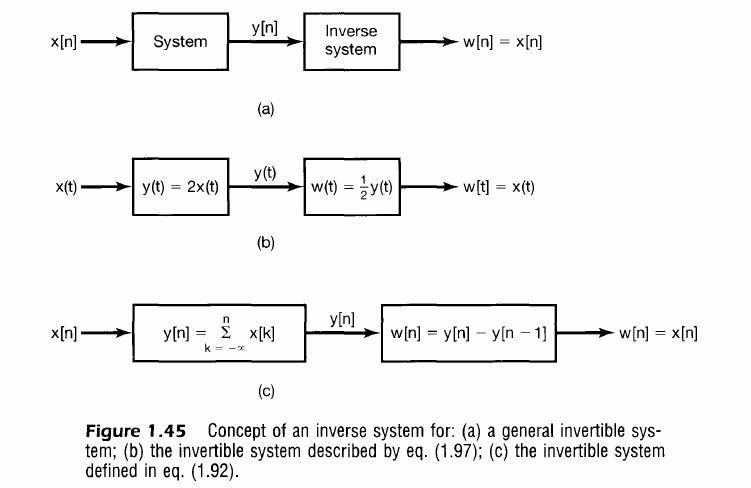
\includegraphics[width=10cm]{a13}
\end{center}
See that the series interconnection between the invertible system and its inverse system has an overall input-output relationship
same as that for the identity system.
As illustrated in the second graph, an example of an invertible
continuous-time system is 
\begin{equation*}
y(t)=2x(t)
\end{equation*}
for which the inverse system is
\begin{equation*}
w(t)=\frac{1}{2}y(t)
\end{equation*}
Another example is illustrated in the third block diagram, see that the accumulator is an invertible system:
\begin{equation*}
y[n]=\sum^n_{k=-\infty}x[k]
\end{equation*}
with inverse system
\begin{equation*}
w[n]=y[n]-y[n-1]
\end{equation*}
Examples of noninvertible systems include
\begin{equation*}
y[n]=0
\end{equation*}
or
\begin{equation*}
y(t)=x^2(t)
\end{equation*}
where a single output can correspond to different inputs.\\
(next page)\newpage
\noindent\textbf{Stability}\\
Another important system property is \textit{stability}. Informally, a stable system is one in which small inputs lead to
responses that do not diverge (grow uncontrollably).\\
\vspace{1mm}\\
More formally, if the input to a stable system is bounded (if its magnitude of the input does not grow without bound), then the
output must also be bounded and therefore cannot diverge. (this is the definition to take note of)\\
\vspace{1mm}\\
For instance consider the averaging system brought up earlier
\begin{equation*}
y[n]=\frac{1}{2M+1}\sum^{+M}_{k=-M}x[n-k]
\end{equation*}
Suppose that the input $x[n]$ is bounded in magnitude by some number, say $B$ for all values of $n$. Then the largest possible 
magnitude for $y[n]$ is also $B$ since it is the average. Therefore, $y[n]$ is bounded and the system is stable.\\
\vspace{1mm}\\
On the other hand, the accumulator sums all of the past values of the input, so the output will grow continually even if $x[n]$
is bounded---it is an unstable system.\\
\vspace{1mm}\\
A useful strategy to verify that a system is unstable is to look for a specific bounded input that leads to an unbounded
output. For instance consider 
\begin{equation*}
y(t)=tx(t)
\end{equation*}
See that a constant input $x(t)=1$ yields $y(t)=t$, which is unbounded. Since for any finite constant bound, $|y(t)|$ will exceed 
that bound at some $t$, this system is unstable.\\
\vspace{1mm}\\
Now consider a different system
\begin{equation*}
y(t)=e^{x(t)}
\end{equation*}
See that for an arbitrary positive number $B$, if $x(t)$ is bound by $B$, that is
\begin{equation*}
|x(t)|<B
\end{equation*}
or
\begin{equation*}
-B<x(t)<B
\end{equation*}
for all $t$, then $y(t)$ must satisfy
\begin{equation*}
e^{-B}<|y(t)|<e^B
\end{equation*}
Any input to this system bounded by an arbitrary positive number $B$ has a output guaranteed to be bounded by $e^B$---this system
is stable.
\newpage

\subsection{Basic system properties 2}
\textbf{Time invariance}\\
A system it \textit{time invariant} if a time shift in the input signal results in an identical time shift in the output
signal.\\
\vspace{1mm}\\
That is, if $y[n]$ is the output of a discrete-time, time-invariant system with input $x[n]$, then $y[n-n_0]$ is the output
when $x[n-n_0]$ is applied. In continuous time with $y(t)$ the output corresponding to the input $x(t)$, a time-invariant system
will have $y(t-t_0)$ as the output when $x(t-t_0)$ is the input.\\
\vspace{1mm}\\
\textbf{Examples}\\
Consider the continuous-time system
\begin{equation*}
y(t)=\sin[x(t)]
\end{equation*}
To check that this system is time invariant, we must determine whether the time-invariance property holds for \textit{any} input
and \textit{any} time shift $t_0$. Thus, letting $x_1(t)$ be an
arbitrary input to the system, with corresponding output
\begin{equation*}
y_1(t)=\sin[x_1(t)]
\end{equation*}
Now consider a second input $x_2$ obtained by shifting $x_1(t)$ in time
\begin{equation*}
x_2(t)=x_1(t-t_0)
\end{equation*}
The output corresponding to this input is
\begin{equation*}
y_2(t)=\sin[x_2(t)]=\sin[x_1(t-t_0)]
\end{equation*}
Now consider translating the output $y_1$, see that
\begin{equation*}
y_1(t-t_0)=\sin[x_1(t-t_0)]
\end{equation*}
Since $y_2$, the output of the shifted input, is the same as $y_1(t-t_0)$, which is if we had shifted the output instead, this
system is time invariant.\\
(next page)\newpage
\noindent\textbf{More examples}\\
As a second example, consider
\begin{equation*}
y[n]=nx[n]
\end{equation*}
See that time shifting the input doesn't correspond with an equivalent shift in the output---this is a time-varying system. 
This system represents one with a time-varying gain, even if we know the input value, we cannot determine the output value 
without knowing the current time.\\
\vspace{1mm}\\
For a counterexample, consider having input $x_1[n]=\delta[n]$, which yields an output $y_1[n]=0$ (since $n\delta[n]=0$). 
However, the input $x_2[n]=\delta[n-1]$ yields the output $y_2[n]=n\delta[n-1]=\delta[n-1]$---while $x_2[n]$ is a shifted 
version of $x_1[n]$, $y_2[n]$ is \textit{not} a shifted version of $y_1[n]$.\\
\vspace{1mm}\\
For a final example, consider the system
\begin{equation*}
y(t)=x(2t)
\end{equation*}
This system represents a time scaling. That is, $y(t)$ is a time-compressed (by a factor of 2) version of $x(t)$.
Intuitively then, any time shift in the input will also be compressed by a factor of 2, and it is for this reason that the system 
is not time invariant. Consider a counterexample: 
\begin{center}
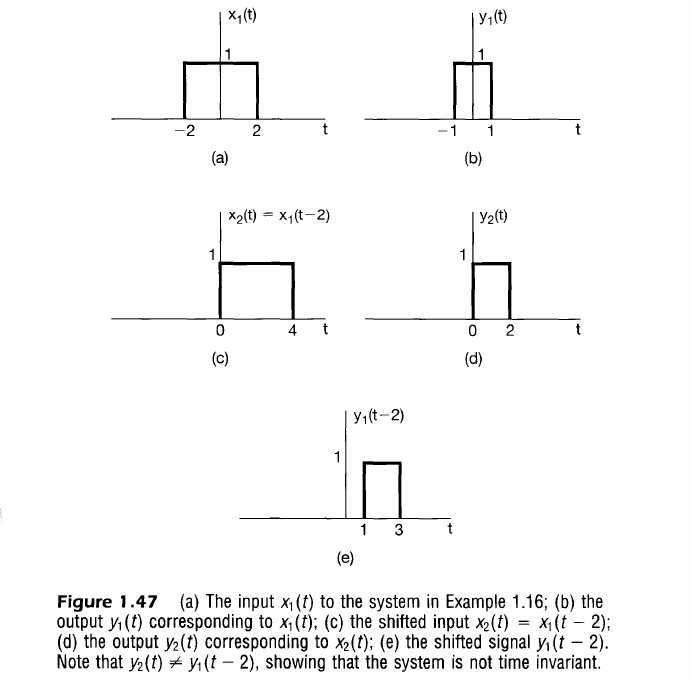
\includegraphics[width=8.5cm]{a14}
\end{center}
see that
if we shift the input signal by 2, the resulting output is not the same as if we had shifted the output signal by 2.\\
(next page)\newpage
\noindent\textbf{Linearity}\\
A \textit{linear system}, in continuous or discrete time, is a system that possesses the important property of superposition: If
an input consists of the weighted sum of several signals, then the output is the superposition---that is, the weighted sum---of
the responses of the system to each of those signals.\\
\vspace{1mm}\\
More precisely, letting $y_1(t)$ be the response of a continuous-time system to an input $x_1(t)$, 
and $y_2(t)$ the response to $x_2(t)$, the system is linear if:
\begin{enumerate}
\item The response to $x_1(t)+x_2(t)$ is $y_1(t)+y_2(t)$.
\item The response to $ax_1(t)$ is $ay(1)$, where $a$ is any complex constant.
\end{enumerate}
The first property is known as the \textit{additivity} propery, while the second the \textit{scaling} or \textit{homogeneity} 
property; the same definition holds for continuous time.
Note that a system can be linear without being time invariant, and it can be time invariant without being linear.\\
\vspace{1mm}\\
The two properties defining a linear system can be combined into a single statement:
\begin{align*}
\text{continuous time: }ax_1(t)+bx_2(t)&\to ay_1(t)+by_2(t)\\
\text{discrete time: }ax_1[n]+bx_2[n]&\to ay_1[n]+by_2[n]
\end{align*}
where $a$ and $b$ are any complex constants.\\
\vspace{1mm}\\
From this see that for a set of inputs $x_k[n],k=1,2,3,\ldots$ to a discrete-time linear system with corresponding outputs 
$y_k[n],k=1,2,3,\ldots$, then the response to a linear combination of these inputs given by 
\begin{equation*}
x[n]=\sum_ka_kx_k[n]=a_1x_1[n]+a_2x_2[n]+a_3x_3[n]+\ldots
\end{equation*}
is
\begin{equation*}
y[n]=\sum_ka_ky_k[n]=a_1y_1[n]+a_2y_2[n]+a_3y_3[n]+\ldots
\end{equation*}
This is known as the \textit{superposition property}, which holds for linear systems in both continuous and discrete time.\\
\vspace{1mm}\\
See that a direct consequence of the superposition property is that, for linear systems, an input which is zero for all time
results in an output which is zero for all time; if $x[n]\to y[n]$, then by the homogeneity property 
\begin{equation*}
0=0\cdot x[n]\to0\cdot y[n]=0
\end{equation*}
(next page)\newpage
\noindent\textbf{Examples}\\
Consider the system
\begin{equation*}
y(t)=tx(t)
\end{equation*}
To determine whether or not it is linear, we consider two arbitrary inputs $x_1(t)$ and $x_2(t)$.
\begin{align*}
x_1(t)&\to y_1(t)=tx_1(t)\\
x_2(t)&\to y_2(t)=tx_2(t)
\end{align*}
Now consider $x_3(t)$, a linear combination of $x_1(t)$ and $x_2(t)$:
\begin{equation*}
x_3(t)=ax_1(t)+bx_2(t)
\end{equation*}
where $a$ and $b$ are arbitrary scalars. See that for input $x_3(t)$, we have the output
\begin{align*}
y_3(t)&=tx_3(t)\\
&=t(ax_1(t)+bx_2(t))\\
&=atx_1(t)+btx_2(t)\\
&=ay_1(t)+by_2(t)
\end{align*}
So we conclude that the system is linear (also see that it is not time invariant).\\
\vspace{1mm}\\
For another example, consider the system
\begin{equation*}
y(t)=x^2(t)
\end{equation*}
as defining $x_1(t),x_2(t)$, and $x_3(t)$ as in the previous example, we have
\begin{align*}
x_1(t)\to y_1(t)=x^2_1(t)\\
x_2(t)\to y_2(t)=x^2_2(t)
\end{align*}
and 
\begin{align*}
x_3(t)\to y_3(t)&=x^2_3(t)\\
&=(ax_1(t)+bx_2(t))^2\\
&=a^2x^2_1(t)+b^2x^2_2(t)+2abx_1(t)x_2(t)\\
&=a^2y_1(t)+b^2y_2(t)+2abx_1(t)x_2(t)
\end{align*}
which isn't a superposition of the inputs, thus the system is not linear.\\
(next page)\newpage
\noindent\textbf{More examples}\\
It is important to remember that the scaling constants of the superposition criteria are allowed to be complex. Consider
the system
\begin{equation*}
y[n]=\text{Re}\{x[n]\}
\end{equation*}
This system is additive, but does not satisfy the homogeneity property, consider input
\begin{equation*}
x_1[n]=r[n]+is[n]
\end{equation*}
the corresponding output is 
\begin{equation*}
y_1[n]=r[n]
\end{equation*}
Now consider scaling $x_1[n]$ by a complex number, for instance $a=i$; defined as $x_2$:
\begin{align*}
x_2[n]&=ix_1[n]=i(r[n]+is[n])\\
&=-s[n]+ir[n]
\end{align*}
The corresponding output then is
\begin{equation*}
y_2[n]=\text{Re}\{x_2[n]\}=-s[n]
\end{equation*}
which is not equal to the scaled version of $y_1[n]$:
\begin{equation*}
ay_1[n]=ir[n]
\end{equation*}
thus the system violates the homogeneity property and is not linear.\\
(next page)\newpage
\noindent\textbf{Example---incrementally linear system}\\
Consider the system
\begin{equation*}
y[n]=2x[n]+3
\end{equation*}
This system is not linear, see that it violates the additivity property:
\begin{align*}
x_1[n]\to y_1[n]=2x_1[n]+3\\
x_2[n]\to y_2[n]=2x_2[n]+3
\end{align*}
where the response to $x_3[n]=x_1[n]+x_2[n]$ is
\begin{equation*}
y_3[n]=2(x_1[n]+x_2[n])+3
\end{equation*}
while 
\begin{equation*}
y_1[n]+y_2[n]=2(x_1[n]+x_2[n])+6
\end{equation*}
See that this system violates the property of linear systems where zero input yields zero output.\\
\vspace{1mm}\\
It may be surprising that the system here is nonlinear since it describes a linear equation. Intuitively, see that the output
of this system can be represented as the sum of the output of a linear system
\begin{equation*}
x[n]\to2x[n]
\end{equation*}
and another signal equal to the \textit{zero-input
response} of the system (when the input is zero), 
\begin{equation*}
y_0[n]=3
\end{equation*}
\begin{center}
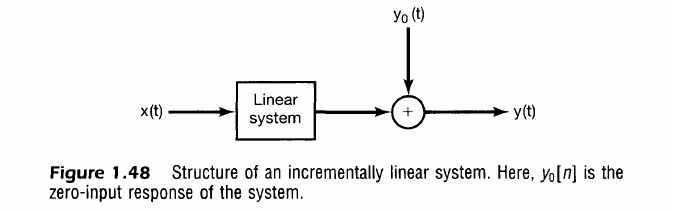
\includegraphics[width=10cm]{a15}
\end{center}
There are large classes of systems that can be represented like this, for which the overall system output
consists of the superposition of the response of a linear system with a zero-input response; these systems correspond to the class
of \textit{incrementally linear systems}.\\
\vspace{1mm}\\
The \textit{difference} between the resposnes to any two inputs to an incrementally system is a 
linear (additive and homogeneous) function of the \textit{difference} between the two inputs. For example, for inputs $x_1[n]$, 
$x_2[n]$ and corresponding outputs $y_1[n]$, $y_2[n]$ we have
\begin{equation*}
y_1[n]-y_2[n]=2x_1[n]+3-(2x_2[n]+3)=2[x_1[n]-x_2[n]]
\end{equation*}
\newpage

\section{Linear Time-Invariant Systems}










\end{document}
